\documentclass[11pt, oneside]{article}   	% use "amsart" instead of "article" for AMSLaTeX format
\usepackage{geometry}                		% See geometry.pdf to learn the layout options. There are lots.
\geometry{letterpaper}                   		% ... or a4paper or a5paper or ... 
%\geometry{landscape}                		% Activate for for rotated page geometry
%\usepackage[parfill]{parskip}    		% Activate to begin paragraphs with an empty line rather than an indent
\usepackage{graphicx}				% Use pdf, png, jpg, or eps� with pdflatex; use eps in DVI mode
								% TeX will automatically convert eps --> pdf in pdflatex		
\usepackage{amssymb}
\usepackage{amsmath}
\usepackage{parskip}
\usepackage{color}
\usepackage{hyperref}

\title{Functions of a complex variable}
%\author{The Author}
%\section{}
%\subsection*{}
\date{}							% Activate to display a given date or no date

\graphicspath{{/Users/telliott_admin/Dropbox/Tex/png/}}
% \begin{center} 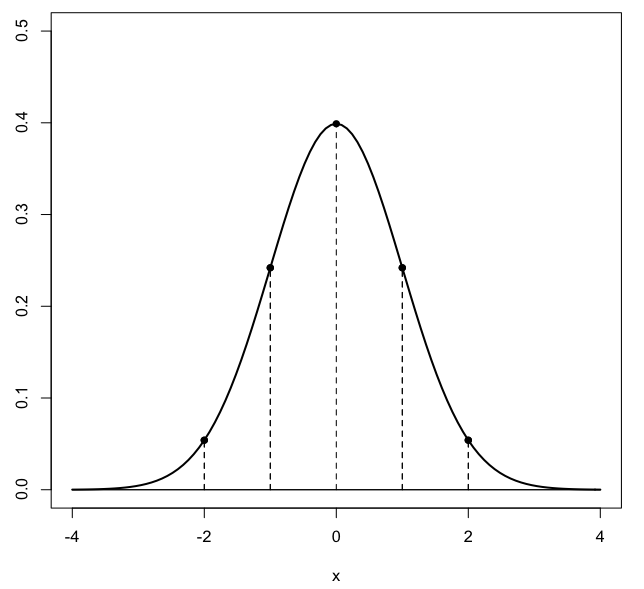
\includegraphics [scale=0.4] {gauss3.png} \end{center}
\begin{document}
\maketitle
\Large
We differentiate and integrate complex functions in a way that is similar to real functions, with these differences:  first, we restrict our attention to functions that are analytic, and we pay attention to points in the complex plane where they have poles (or singularities).  Second, the integrals that we compute are line integrals.  Let's do one.

\subsection*{example}

In general terms, if we have
\[ z = x + i y \]
\[ dz = dx + i dy \]
and the function
\[ w = f(z) \]
\[ = u(x,y) + iv(x,y) \]
we can write either
\[ \int f(z) \ dz = \int (x + i y) (dx + i dy) \]
or what may be less confusing:
 \[ \int f(z) \ dz = \int (u + i v) (dx + i dy) \]
\[ = \int u \ dx - \int v \ dy + i \ [ \ \int v \ dx + \int u \ dy \ ] \]

Just as with line integrals for real functions of $x$ and $y$, this is \emph{not} some kind of double integral in both variables.

Recall that for the work integral
\[ \int_C \mathbf{F} \cdot d \mathbf{r} = M \ dx + N \ dy \]
we parametrize the curve to get the integral over a single variable.

Suppose our function is simply $z = x + iy$.  The integral is 
\[ \int z \ dz = \int (x + iy) (dx + i dy) \]
\[ = \int x \ dx - y \ dy + i x \ dy + i y \ dx \]

Now we must get $y$ in terms of $x$ from the curve.  Suppose the curve goes from $(1,i)$ to $(3,i)$, then to $(3,3i)$ and finally back to where we started.  

We have three segments.  Along the first part, we are moving in the positive $x$ direction, with no change in $y$, so $dy=0$ and $y = 1$, a constant, and the integral is
\[ \int x \ dx - y \ dy + i x \ dy + i y \ dx \]
\[ = \int x \ dx + i y \ dx \]
\[ = \int_{x=1}^{x=3} \ x + i  \ dx \]
\[ = \frac{x^2}{2} + ix \ \bigg |_1^3 \]
\[ = 4 + 2i \]

Along the second part, we are moving in the positive $y$ direction with $dx = 0$ and $x = 3$ so
\[ \int x \ dx - y \ dy + i x \ dy + i y \ dx \]
\[ = \int y_{y=1}^{y=3} - y \ dy + 3 i \ dy \]
\[ = -\frac{y^2}{2} + 3iy \ \bigg |_1^3 \]
\[ = -4 + 6i \]

And for the third, we have that both $dx$ and $dy$ are non-zero, so we must actually do the parametrization.  The curve is $y=x$.  Hence $dy = dx$.
\[ \int x \ dx - y \ dy + i x \ dy + i y \ dx \]
\[ \int x \ dx - x \ dx + i x \ dx + i x \ dx \]
Suppose we take the path as going from $(1,1)$ to $(3,3)$.
\[ = 2i \int_{x=1}^{x=3} x \ dx \]
\[ = 2i \ \frac{x^2}{2} \ \bigg |_1^3 \]
\[ = 2i \ \frac{8}{2} = 8i \]
Notice that 
\[ \int_{C1} + \int_{C2} = \int_{C3} = 8i \]
Alternatively, if we follow the curve $C3$ from $(3,3)$ to $(1,1)$, the whole thing is just zero.  We will see later that this is not a coincidence.

\subsection*{example}
As a second example, consider $f(z) = z^2$.  For the path, take the unit circle over the first quadrant from $(1,0)$ to $(0,1)$.  There is an easy way to do this, and a hard way.  Let's start with the hard way.

Write $z$ in terms of $x$ and $y$:
\[ z = x + iy \]
\[ z^2 = x^2 - y^2 + 2ixy \]
Also
\[ dz = dx + i \ dy \]
So
\[ \int z^2 \ dz = \int (x^2 - y^2 + 2ixy) ( dx + i \ dy) \]
\[ = \int (x^2 - y^2) \ dx - \int 2 xy \ dy + i \int 2xy \ dx + i \int (x^2-y^2) \ dy \]
As before, we must parametrize this using the relationship between $x$ and $y$ along the curve.
\[ x = \cos t \]
\[ y = \sin t \]
\[ dx = - \sin t \ dt \]
\[ dy = \cos t \ dt \]
and then
\[ x^2 - y^2 = \cos^2 t - \sin^2 t = \cos 2t \]
\[ 2xy = 2 \cos t \sin t = \sin 2t \]
so the integral is
\[ = \int -\cos 2t \  \sin t \ dt - \int \sin 2t \ \cos t \ dt + \dots \]
\[ + \ i \ [ \ \int - \sin 2t \ \sin t \ dt + \int \cos 2t \ \cos t \ dt \]

Looks pretty wild!  In the book they use some trig identities I hadn't seen before, namely starting with the standard
\[ \sin s + t = \sin s \cos t + \sin t \cos s  \]
\[ \cos s + t = \cos s \cos t - \sin s \sin t \]
then, if $s = 2t$ then
\[ \sin 3t = \sin 2t \cos t + \sin t \cos 2t \]
\[ \cos 3t = \cos 2t \cos t - \sin 2t \sin t \]
Looking at the real part of the integral we had (combining terms)
\[ \int -\cos 2t \  \sin t - \sin 2t \ \cos t \ dt = \int - \sin 3t \ dt = \frac{\cos 3t}{3} \]
and for the imaginary part of the integral
\[ i \ [ \ \int - \sin 2t \ \sin t + \cos 2t \ \cos t \ dt = i \int \cos 3t \ dt = i \frac{\sin 3t}{3} \]
That looks a lot better.
\[ \frac{\cos 3t}{3} + i \frac{\sin 3t}{3} \ \bigg |_0^{\pi/2} = - \frac{1}{3} - i \frac{1}{3} = - \frac{1}{3} (1 + i) \]

For the easy way, just treat $z$ as if it were a real variable
\[ \int z^2 \ dz = \frac{z^3}{3} \ \bigg |_1^i = - \frac{1}{3} i - \frac{1}{3} \]
Note that if we go all the way around the unit circle the integral is just zero.

Going back to the first example we had
\[ \int z \ dz = \frac{z^2}{2} \ \bigg |_{1 + i}^{3 + 3i} \]
\[ = \frac{9 - 9 + 18i - \ [ \ 1 - 1 + 2i \ ] }{2} \]
\[ = 8i \]

\subsection*{example}
\[ \int_0^{2\pi} \frac{1}{z} \ dz \]
If we are on the unit circle, then 
\[ z = e^{i\theta} \]
\[ dz = ie^{i\theta} d \theta \]
\[ \int \frac{dz}{z} = \int e^{-i\theta} \ i  e^{i \theta} \ d \theta = 2 \pi i \]

If we're centered on the origin but we don't have a unit circle, there will be an $r$ in both the numerator and the denominator, which cancel.  The result is thus independent of the radius of the circle.

In general
\[ \oint_C \frac{dz}{(z - z_0)^n} = 
\begin{cases}
0, & n \ne 1 \\
2 \pi i, & n = 1 
\end {cases}
\]

Examining the inverse function a little further, let's confirm that it is analytic by calculating the partial derivatives.  We have
\[ \frac{1}{z} = \frac{1}{x + iy} \]
One way to simplify is to multiply on top and bottom by $z*$:
\[ = \frac{1}{x + iy} \ \frac{x-iy}{x- iy} \]
\[ = \frac{x - iy}{x^2 + y^2} \]
Thus
\[ u = \frac{x}{x^2 + y^2} \]
\[ u_x = \frac{(x^2 + y^2) - 2x^2}{(x^2 + y^2)^2} = \frac{y^2 - x^2}{(x^2 + y^2)^2} \]
\[ u_y = \frac{-2xy}{(x^2 + y^2)^2} \]
And
\[ v =  \frac{-y}{x^2 + y^2} \]
\[ v_y = - \frac{(x^2 + y^2) - 2y^2}{(x^2 + y^2)^2} = \frac{y^2 - x^2}{(x^2 + y^2)^2} \]
\[ v_x = \frac{2xy}{(x^2 + y^2)^2} \]
CRE are satisfied and the inverse of $z$ is analytic.

Note that if we integrate the same function explicitly in terms of $x$ and $y$, say, around a unit square, we run into problems.  First let's  do $[0,0 \times 1,1]$.  We have
\[ \int u \ dx - \int v \ dy + i \ [ \ \int v \ dx + \int u \ dy \ ]  \]
Along $C1$, $y = 0$ and $dy = 0$ so:
\[ \int \frac{x}{x^2 + y^2} \ dx + i \ [ \ \int \frac{-y}{x^2 + y^2} \ dx \]
\[ = \int_0^1 \frac{1}{x} \ dx = \ln x \ \bigg |_0^1 \]
Since $\ln 0$ is not defined, we can't do this.

\subsection*{example}
We can extend this to 
\[ \oint \frac{dz}{z^2} \]
As before, on the unit circle
\[ z = e^{i\theta} \]
\[ dz = i z \ d \theta \]
so the integral is
\[ \int_0^{2 \pi} \ \frac{i}{z} \ d \theta =  \int_0^{2 \pi} i e^{-i\theta} \ d \theta \]
\[ = i \frac{1}{-i} e^{-i\theta} \ \bigg |_0^{2 \pi} = e^{-2\pi i} - e^0 \]
Evaluate the first term using Euler's formula:
\[ e^{-2\pi i} = \cos -2 \pi + i \sin -2 \pi = 1 \]
So the whole thing is zero.

\end{document}  